\problemname{Robottävling}
\noindent
You have built a robot for a robot competition. One of the tasks the robot
must solve is to count the number of cubes in a square grid.
The grid has $N$ rows and $N$ columns, and in each cell there is a
stack of $1$ to $5$ identical cubes.
Unfortunately, your robot is not very good at collecting information.
The only thing it can do is find the height of the tallest stack in each row and column.
You had planned to compensate for this by making the robot very smart.
Write a program that, given the information the robot collected,
computes the minimum and maximum possible number of cubes in the grid.

\section*{Input}
The first line contains an integer $N$ $(3 \le N \le 10)$, the number of rows and columns in the grid.
The second line contains $N$ integers $r_i$ $(1 \leq r_i \leq 5)$,
the height of the tallest stack in row $i$. The third line contains $N$ integers
$c_i$ $(1 \leq c_i \leq 5)$, the height of the tallest stack in column $i$.
It is guaranteed that there are no contradictions in the input,
that is, there will always exist at least one valid placement
of cubes that produces the given values.

\section*{Output}
The program should print two integers: the minimum possible and the maximum possible total number of cubes in the grid.


\section*{Scoring}
\noindent
\begin{tabular}{| l | l | p{12cm} |}
  \hline
  \textbf{Group} & \textbf{Points} & \textbf{Constraints} \\ \hline
  $1$    & $20$       & $N=3$ and you only need to get the maximum number of cubes correct. \\ \hline
  $2$    & $20$       & You only need to get the maximum number of cubes correct. \\ \hline
  $3$    & $20$       & $N=3$ \\ \hline
  $4$    & $40$       & No additional constraints \\ \hline
\end{tabular}


\section*{Explanation of Sample}
\begin{figure}[!h]
  \centering
      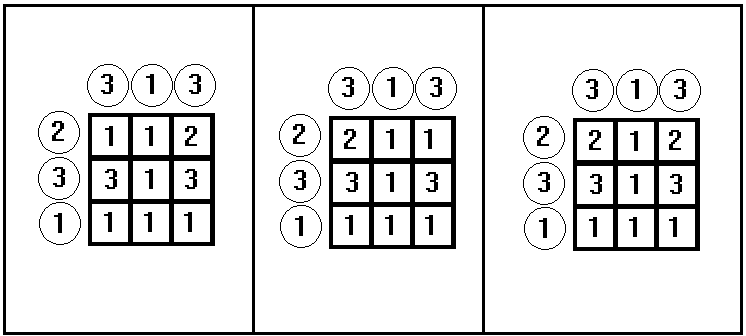
\includegraphics[width=.5\textwidth]{robotbild.png}
\end{figure}
These three are the only possible configurations for the first sample. Both of the first two have a total of 14 cubes and the third has a total of 15 cubes. The answer is thus that the minimum possible total number of cubes is 14, and the maximum possible is 15.
